\chapter{Исследование существующих алгоритмов построения выпуклых оболочек} \label{chapt1}

\section{Существующие алгоритмы построения выпуклых оболочек} \label{sect1_1}

За долгое время развития вычислительной геометрии появилось огромное количество алгоритмов. Они имеют различную сложность и принцип работы. Необходимо исследовать эти алгоритмы, чтобы понимать какой алгоритм нам нужно будет сделать, чтобы с ними соперничать.

Все алгоритмы будут рассмотрены в препдположении, что все точки находятся в общем положении. Это означает, что никакие три точки не лежат на одной прямой. Это сделано только для упрощения выкладок, на практике конечно необходимо учитывать этот случай и он может быть учтён всеми представленными алгоритмами.

Также необходимо ввести предикат $ccw(A, B, C)$, который также будет использоваться для описания алгоритмов. Предикат $ccw$ показывает точки $A, B, C$ перечислены в порядке против часовой стрелки или нет. Другими словами точка $C$ должна лежать левее прямой $A, B$. На рисунке~\ref{img:ccw_1} показано, что предикат для точек $A, B, C$ выполняется, а на рисунке~\ref{img:ccw_2} он выполняться не будет.

\begin{figure}[ht]
	{\centering
		\hfill
		\subbottom[\label{img:ccw_1}]{%
			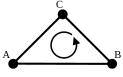
\includegraphics[width=0.4\linewidth]{ccw1}}
		\hfill
		\subbottom[\label{img:ccw_2}]{%
			\includegraphics[width=0.4\linewidth]{ccw2}}
		\hfill
	}
	\caption{Демонстрация работы предиката $ccw$}
	\label{img:ccw}
\end{figure}

Предикат $ccw$ вычисляется очень просто. Сначала необходимо посчитать детерминант $det$ матрицы \eqref{eq:det}.

\begin{equation}\label{eq:det}
det(A, B, C)= \left| \begin{array}{ccc} x_A & y_A & 1 \\ x_B & y_B & 1 \\ x_C & y_C & 1  \end{array}\right|
\end{equation}

Теперь можно определить $ccw$ через $det$ \eqref{eq:ccw}.

\begin{equation}\label{eq:ccw}
ccw(A, B, C)=det(A, B, C) > 0
\end{equation}


\subsection{Алгоритм Джарвиса} \label{subsect1_1_1}

Алгоритм Джарвиса - это один из первых придуманных алгоритмов построения выпуклой оболочки. Он был опубликован в 1972 году. %TODO ref
Этот алгоритм также называют алгоритмом заворачивания подарка, что отлично показывает суть работы алгоритма.

Пусть нам дано множество точек $S$. Первым делом нам надо найти такую точку $t$, чтобы было известно, что она будет лежать на выпуклой оболочке. Самый простой способ сделать это - найти левую крайнюю точку. Не теряя общности рассуждений, примем найденную точку за $t_0$. Алгоритм начинает работать при $i=0$ в точке $t_0$ и выбирает такую точку $t_{i+1}$ такую, что все остальные точки лежат правее прямой $t_i, t_{i+1}$. Также это выражается с помощью предиката \eqref{eq:ccw}:
\[
\forall p \in S \backslash \{t_i, t_{i+1}\} : ccw(t_i, t_{i+1}, p)
\]

Прямая $t_i, t_{i+1}$ на первых шагах алгоритма показана на рисунке ~\ref{img:jarvis}. Повторение этого действия пока не $t_h=p_0$ полностью построит выпуклую оболочку изначально заданного множества.

\begin{figure}[ht]
    {\centering
        \hfill
        \subbottom[\label{img:jarvis_1}]{%
            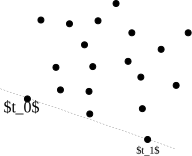
\includegraphics[width=0.4\linewidth]{jarvis1}}
        \hfill
        \subbottom[\label{img:jarvis_2}]{%
            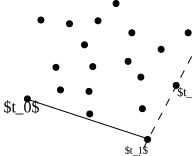
\includegraphics[width=0.4\linewidth]{jarvis2}}
        \hfill
    }
    \caption{Первые этапы работы алгоритма Джарвиса}
    \label{img:jarvis}
\end{figure}

Какова сложность алгоритма Джарвиса? Если в множестве изначально было $n$ точек, а в выпуклую оболочку попало ровно $h$ точек, то сложность алгоритма заворачивания подарка равна $O(nh)$. Доказательство этого утверждения очевидно. Так как поиск точки $t_{i+1}$ занимает проход по всему множеству точек, то это имеет сложность $O(n)$. Всего нам необходимо найти $h$ точек, так как именно столько будет находится в выпуклой оболочке.

Как видно из сложности алгоритма, он зависит не только от входных данных, но и от выходных. Это интересная особенность алгоритмов построения выпуклых оболочек, хоть и не все из них имеют сложность, зависящую от выходных данных.

\subsection{Алгоритм Грэхема} \label{subsect1_1_2}
